\chapter{System Design}

\section{System Architecture and Block Diagram}
SecureSphere-AI is designed as an asynchronous, zero-trust security reverse proxy operating at the network perimeter between internal enterprise clients and external cloud LLM providers. The architecture comprises two principal decoupled processes:
\begin{enumerate}[leftmargin=*]
    \item \textbf{The Core Gateway Service (\texttt{gateway/main.py}):} An asynchronous FastAPI proxy executing on port 8000 that orchestrates policy enforcement, entity extraction, cryptographic tokenization, homomorphic math evaluation, and response de-anonymization.
    \item \textbf{The Enterprise SOC Dashboard (\texttt{dashboard/app.py}):} A Streamlit control center running on port 8501 providing real-time telemetry, cryptographic verification sandboxes, multimodal screenshot redactors, and security audit logs.
\end{enumerate}

\begin{figure}[H]
    \centering
    \IfFileExists{images/architecture_diagram.png}{%
        \includegraphics[width=\textwidth]{images/architecture_diagram.png}%
    }{%
        \IfFileExists{architecture_diagram.png}{%
            \includegraphics[width=\textwidth]{architecture_diagram.png}%
        }{%
            \framebox[\textwidth]{\rule{0pt}{7cm}\textbf{Figure 3.1: SecureSphere-AI System Architecture Diagram}}%
        }%
    }
    \caption{SecureSphere-AI Dual-Phase Zero-Trust System Architecture}
    \label{fig:architecture}
\end{figure}

\subsection{Architectural Layer Decomposition}
The gateway processing pipeline is partitioned into four functional layers:
\begin{itemize}[leftmargin=*]
    \item \textbf{Ingress Mediation Layer:} Intercepts REST requests, enforces API key authentication (\texttt{X-API-Key}), sliding-window rate limiting (60 requests/minute), and evaluates inbound prompt injection risks.
    \item \textbf{Contextual Analysis and Scheduling Layer:} Runs Microsoft Presidio, spaCy models, 15+ custom regular expression recognizers, and the greedy interval span scheduler to extract and isolate non-overlapping sensitive entities.
    \item \textbf{Cryptographic and Transformation Layer:} Generates keyed HMAC-SHA256 Base32 pseudonym tokens for text entities, stores mappings in the local authenticated AES-256-GCM session vault, and encrypts numerical monetary figures into TenSEAL CKKS ciphertext tokens.
    \item \textbf{Egress and Restoration Layer:} Injects token preservation system instructions into cloud payloads, dispatches sanitized prompts to Google Gemini or OpenAI, validates outbound responses for toxicity and accidental token leakage, evaluates homomorphic mathematical directives on ciphertexts, and performs client-side de-anonymization.
\end{itemize}

\section{Module Descriptions}

\subsection{Module 1: Inbound Policy and Threat Interceptor}
\begin{itemize}[leftmargin=*]
    \item \textbf{Input:} Raw user prompt text and client metadata.
    \item \textbf{Functionality:} Scans for known prompt-injection signatures, adversarial roleplay prompts (e.g., ``DAN mode'', ``developer mode override''), and high-risk keyword combinations (e.g., banking credentials paired with wire transfer instructions). Computes an inbound toxicity score ($0.0 \le T \le 1.0$).
    \item \textbf{Output:} Boolean allow/block flag, risk score, and detailed block reason if the toxicity threshold ($T \ge 0.80$) is exceeded.
\end{itemize}

\subsection{Module 2: Hybrid Entity Recognition Engine and Interval Scheduler}
\begin{itemize}[leftmargin=*]
    \item \textbf{Input:} Allowed inbound prompt string.
    \item \textbf{Functionality:} Executes Microsoft Presidio Analyzer with spaCy \texttt{en\_core\_web\_sm} alongside 15+ custom recognizers. When enabled via \texttt{ENTITY\_ENGINE=spacy\_bert}, executes sliding-window chunked inference using \texttt{dslim/bert-base-NER}. Passes all candidates to \texttt{filter\_overlapping\_results} to resolve boundary collisions.
    \item \textbf{Output:} Sorted list of validated, non-overlapping \texttt{RecognizerResult} objects containing entity types, confidence scores, and character boundary indices.
\end{itemize}

\subsection{Module 3: Dual Cryptographic Engine}
\begin{itemize}[leftmargin=*]
    \item \textbf{Input:} Raw entity substrings and entity categories.
    \item \textbf{Functionality:} 
    \begin{itemize}
        \item For text, identity, and credential entities: Generates deterministic tokens using \texttt{DeterministicHMACPseudonymizer} and encrypts the mapping inside \texttt{AES256GCMTokenVault} using fresh 96-bit random nonces.
        \item For financial, currency, and numerical figures: Initializes an ephemeral CKKS session via \texttt{ckks\_engine.py}, encrypts numbers into public context ciphertexts, and outputs ciphertext tokens formatted as \texttt{[CKKS\_NUM\_<session>\_<id>]}.
    \end{itemize}
    \item \textbf{Output:} Fully sanitized prompt string, in-memory vault dictionary, and appended instruction notes.
\end{itemize}

\subsection{Module 4: Cloud Router and System Note Injector}
\begin{itemize}[leftmargin=*]
    \item \textbf{Input:} Sanitized prompt string and routing configuration (\texttt{BYPASS\_PII\_ROUTING}).
    \item \textbf{Functionality:} Analyzes the prompt for cryptographic tokens. If tokens are present, injects a system-level preservation rule (\texttt{placeholder\_note()}). Dispatches the payload to Google Gemini 2.5 Flash, OpenAI GPT-4o, or routes to an offline local Ollama model if strict air-gapping is mandated.
    \item \textbf{Output:} Raw LLM response string containing mathematical directives or pseudonym tokens.
\end{itemize}

\subsection{Module 5: Multimodal Computer Vision Guardrail}
\begin{itemize}[leftmargin=*]
    \item \textbf{Input:} Uploaded image byte stream (PNG, JPEG) and redaction mode selection.
    \item \textbf{Functionality:} Decodes image into an OpenCV matrix. Applies HSV/YCrCb color-space segmentation and morphological closing for face detection, and horizontal Sobel gradient filtering with Otsu thresholding for license plates. Applies Gaussian blurring (Mode A) or black-box badge redaction (Mode B).
    \item \textbf{Output:} Sanitized image byte stream and visual detection telemetry.
\end{itemize}

\subsection{Module 6: Outbound Response Validator and De-Anonymizer}
\begin{itemize}[leftmargin=*]
    \item \textbf{Input:} Raw response from the cloud LLM and session vault mapping.
    \item \textbf{Functionality:} Scans response for toxic content and unintentional credential leakage. If the response contains CKKS mathematical directives (e.g., \texttt{CKKS\_SUM}), evaluates them on encrypted ciphertexts and decrypts the result. Finally, executes reverse substitution of all public HMAC tokens from the session vault.
    \item \textbf{Output:} Final de-anonymized, clean text presented to the corporate user.
\end{itemize}

\subsection{Module 7: Autonomous Hybrid Database Logger}
\begin{itemize}[leftmargin=*]
    \item \textbf{Input:} Transaction audit metadata (timestamps, prompt hashes, entity types detected, model used, latency, toxicity score).
    \item \textbf{Functionality:} Attempts logging to primary MongoDB document store. If MongoDB is unreachable (2-second connection timeout), automatically catches the error and persists the audit record into a local SQLite database (\texttt{securesphere.db}).
    \item \textbf{Output:} Immutable, compliant audit trail record.
\end{itemize}

\section{Project Plan and Execution Schedule}
The project was executed following the Agile Software Development Life Cycle (SDLC) over a 16-week timeline, as detailed in Table~\ref{tab:project_plan}.

\begin{table}[htbp]
\centering
\caption{Project Execution Schedule and SDLC Phases}\label{tab:project_plan}
\begin{tabular}{lllc}
\toprule
\textbf{Phase} & \textbf{SDLC Activity} & \textbf{Deliverables} & \textbf{Duration} \\
\midrule
Phase 1 & Literature Survey \& Requirements & Problem formulation, statutory review & Weeks 1--2 \\
Phase 2 & Architectural Design \& Threat Modeling & Reverse proxy topology, sequence models & Weeks 3--4 \\
Phase 3 & Inbound PII Engine Development & Presidio, custom regexes, interval scheduler & Weeks 5--6 \\
Phase 4 & Cryptographic Engine Implementation & HMAC-SHA256, AES-GCM local vault & Weeks 7--8 \\
Phase 5 & TenSEAL CKKS Homomorphic Integration & Real CKKS engine, ciphertext math directives & Weeks 9--10 \\
Phase 6 & Multimodal Vision Guardrail & OpenCV skin-tone \& Sobel plate filters & Weeks 11--12 \\
Phase 7 & System Integration \& Dashboard UI & FastAPI proxy, Streamlit SOC console & Weeks 13--14 \\
Phase 8 & Verification, Testing \& Documentation & 51 unit tests, benchmark evaluation & Weeks 15--16 \\
\bottomrule
\end{tabular}
\end{table}
